%----------------------------------------------------------
\subsection{Data Concept}

Source-Term objects (ST-O $\rightarrow \, \textbf{b}$) are required for the equation system
(EQS).
\begin{eqnarray}
\textbf{A}
\textbf{x}
=
\textbf{b}
\end{eqnarray}
%
The interface between ST-O and EQS objects is the source term
matrix (ST-OM).
Source terms are independent objects, whereas source term
matrices as well as equation systems are model dependent
structures.
% *** EPS-Grafik ***
\begin{figure}[htb!]
\begin{center}
\footnotesize
%\psfrag{Synonym}[pos][pos]{Tex-Ersetzung}
%\psfrag{x}[][]{$t$}
%\psfrag{y}[b][t]{$y(t)$}
%\psfrag{t}[][]{ }
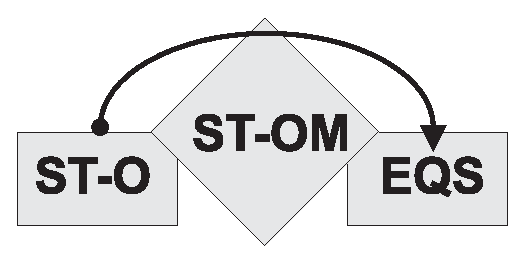
\includegraphics[width=0.4\columnwidth]{figures/ob_st.eps}  % Filename.eps
\caption{Data transfer between source objects and equation system}
\label{fig:st1}
\end{center}
\end{figure}
%


%----------------------------------------------------------
\subsubsection{Source Term Object -- \fbox{ST-O}}

\paragraph{Object Data}

\footnotesize
\begin{verbatim}
typedef struct {
    char *name;
    long type;
    long mode;
    long kind;
    long curve;
    int index;
    long level;
    long begin_node;
    long end_node;
    long step_nodes;
    long begin_element;
    long end_element;
    long step_elements;
    long count_of_values;
    double *values;
    long count_of_points;
    double *x;
    double *y;
    double *z;
    double radius;
    double epsilon;
    long distribution_type;
    int component_number;
    long *nodes;
    int function_nidx;
    char polyline_name[MAX_ZEILE];
} SOURCE_SINK;
\end{verbatim}
\normalsize

\subsubsection*{Object ID}

\subsubsection*{Object Construction}

From RFD file:
\small
\begin{verbatim}
int FctSourcePhaseNew ( ... char *name ... )
int FctSourceMixtureNew ( ... char *name ...)
\end{verbatim}
\normalsize

Interactively by GUI dialog:
\small
\begin{verbatim}
void CSources::OnButtonSSAdd()
  ss = AddSourceSinkObject(ss_name);
void CSources::OnButtonSSRemove()
  DestroySourceSinkObject(nSel,ss_name);

Groups:
int DestroySourceSinkListGroup(char *name)
\end{verbatim}
\normalsize

\subsubsection*{Object Access}

\small
\begin{verbatim}
void CSources::Get_RF2Dialog_ObjectGroup(void)
CString CSources::Get_RF2Dialog_Object(SOURCE_SINK *ss)
  SOURCE_SINK *GetSourceSinkGroup(char *name,SOURCE_SINK *ss)
  SOURCE_SINK *GetSourceSinkObject(long count, char *name)

Groups:
void CSources::Set_Dialog2RF_Object(SOURCE_SINK *ss)
\end{verbatim}
\normalsize



%----------------------------------------------------------
\subsubsection{Source Term Object List -- \fbox{ST-OL}}

\subsubsection*{List Data}

% *** EPS-Grafik ***
\begin{figure}[htb!]
\begin{center}
\footnotesize
%\psfrag{Synonym}[pos][pos]{Tex-Ersetzung}
%\psfrag{x}[][]{$t$}
%\psfrag{y}[b][t]{$y(t)$}
%\psfrag{t}[][]{ }
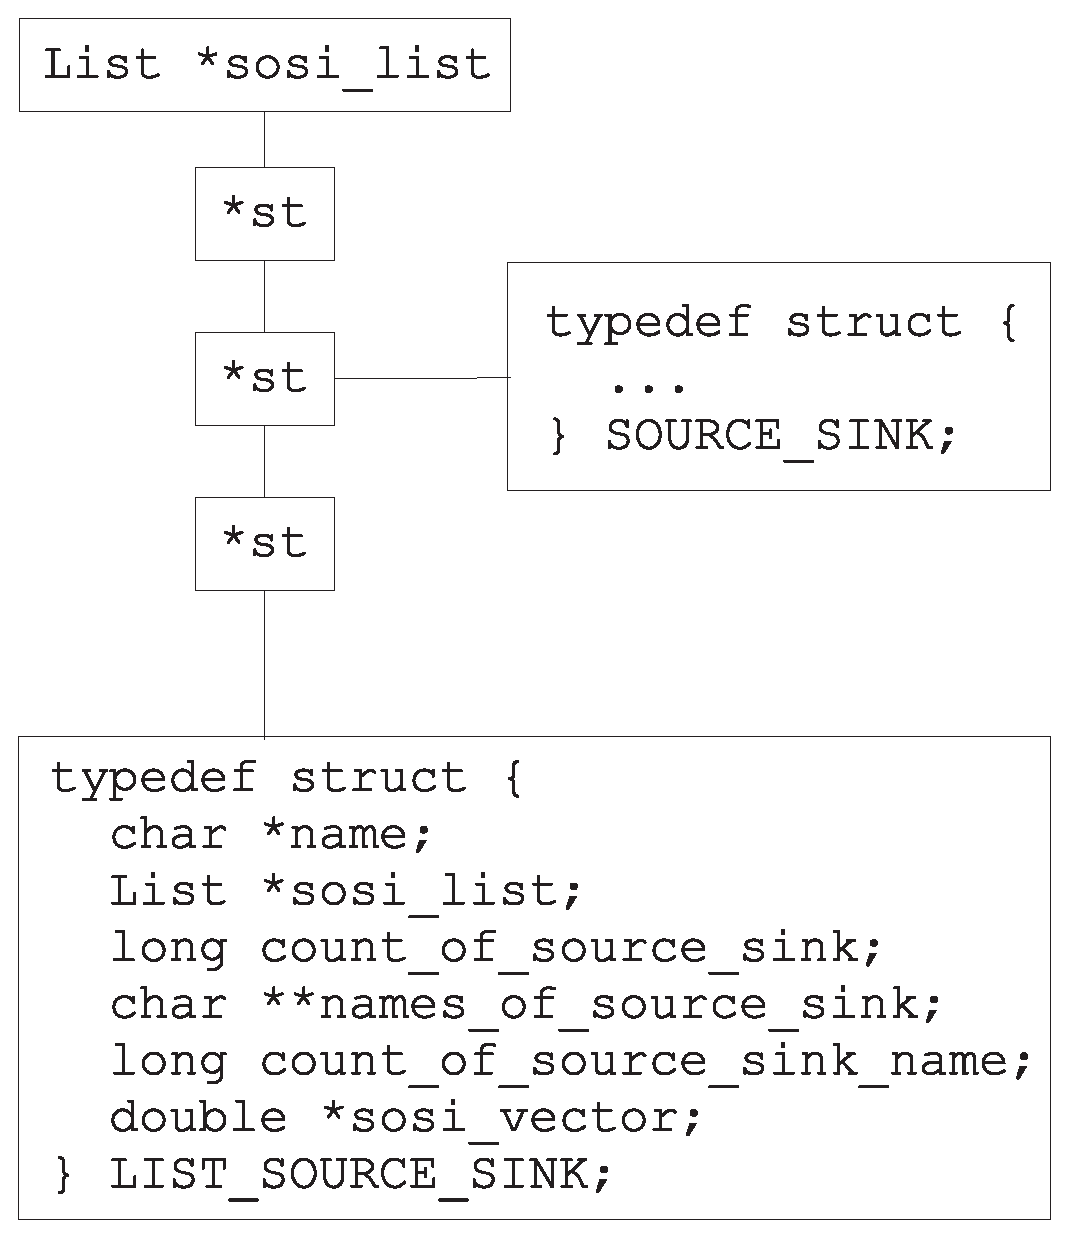
\includegraphics[width=0.4\columnwidth]{figures/st_list.eps}  % Filename.eps
\caption{Source term object list \fbox{ST-OL}}
\label{fig:st_list}
\end{center}
\end{figure}
%

\subsubsection*{List Construction}

\small
\begin{verbatim}
void CreateSourceSinkList(void)
void DestroySourceSinkList(void)
\end{verbatim}
\normalsize


%----------------------------------------------------------
\subsection{Source Term - Object Matrix -- \fbox{ST-OM}}

Source term matrices (ST-OM) are model dependent structures,
building the interface of source term objects to equation systems.
The number of ST-OM columns corresponds to the number of specified ST groups
(e.g. number of unknown functions).
The number of ST-OM rows corresponds to the number of nodes.
ST groups, i.e. ST-O belonging to a unknown function are specified by their name:
\small
\begin{verbatim}
SetSourceSink(name_source_term_group);
\end{verbatim}
\normalsize

\subsubsection*{Matrix Data}

\subsubsection*{Matrix Construction}


%----------------------------------------------------------
\subsection{Source Term - Object Linking}

\subsubsection*{Link to \textsf{EQS}}

%----------------------------------------------------------
\subsection{Source Terms Implementation}

%----------------------------------------------------------
\subsection{Source Term Menu Implementation}
